\section{Auswertung}

Die in der Auswertung bestimmten Ausgleichsrechnungen werden mit
der Funktion \emph{curve\_ fit} \cite{scipy} aus dem Python Paket \emph{scipy.optimize}\cite{scipy} durchgeführt.

\subsection{Auswertung der $T_{00}$ Mode}
\FloatBarrier
In der Tabelle \ref{tab: T_00} befinden sich die aufgenommenen Messwerte.
\begin{table} 
\centering 
\caption{Messwerte der T_00 Mode.} 
\label{tab: T_00} 
\begin{tabular}{S S } 
\toprule  
{$r / \si{ \milli\meter }$} & {$I_p / \si{ \micrompere}$} \\ 
\midrule  
-10.0 & 2.2\\ 
-9.0 & 3.1\\ 
-8.0 & 3.9\\ 
-7.0 & 5.0\\ 
-6.0 & 6.2\\ 
-5.0 & 7.4\\ 
-4.0 & 8.4\\ 
-3.0 & 9.4\\ 
-2.0 & 9.4\\ 
-1.0 & 9.2\\ 
0.0 & 8.8\\ 
1.0 & 8.1\\ 
2.0 & 7.2\\ 
3.0 & 6.1\\ 
4.0 & 5.0\\ 
5.0 & 3.8\\ 
6.0 & 2.7\\ 
7.0 & 1.9\\ 
8.0 & 1.2\\ 
9.0 & 0.7\\ 
10.0 & 0.4\\ 
\bottomrule 
\end{tabular} 
\end{table}
Weiterhin werden die Messdaten in Abbildung \ref{fig: T_00} grafisch dargestellt.
\begin{figure}[h!]
  \centering
  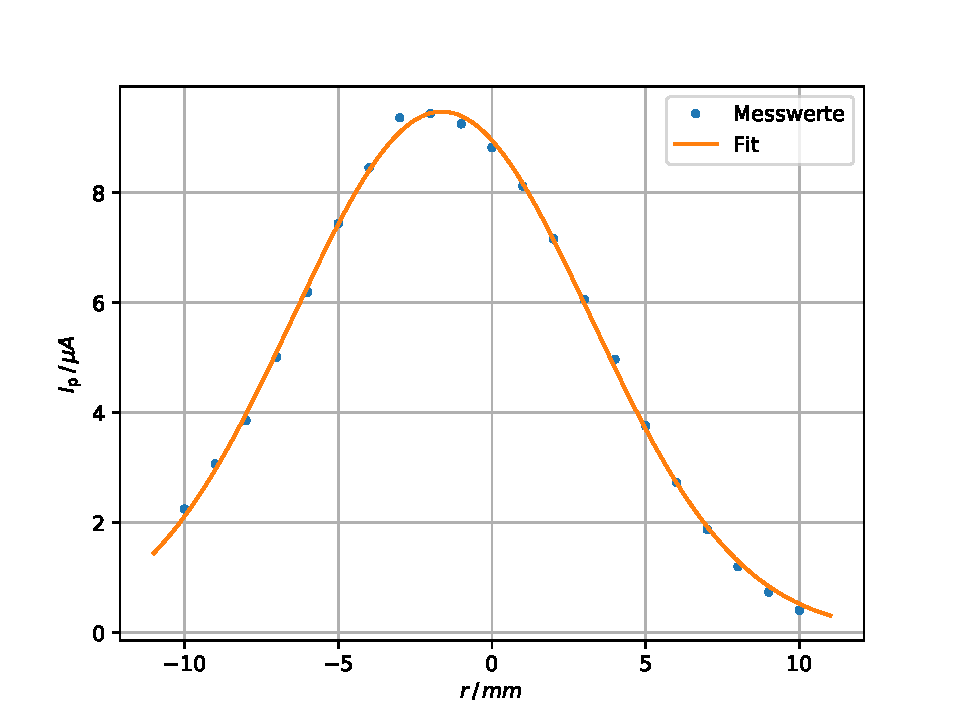
\includegraphics[width=0.7\textwidth]{../Messdaten/plots/T_00.pdf}
  \caption{Plot der in Tabelle \ref{tab: T_00} gelisteten Messwerte. Zusätzlich ist in der Grafik die bestimmte Ausgleichsgeraden zu sehen.}
  \label{fig: T_00}
\end{figure}
In der Abbildung ist die mit Hilfe von \emph{scipy.optimize} an die Funktion \eqref{} erstellte Funktion zu erkennen.
Aus der Ausgleichsrechnung ergeben sich die folgenden Parameter

\begin{align}
  \label{eq: fit_t_00}
  \begin{aligned}
  I_0&=\SI{9.47 \pm 0.05}{\micro\ampere}\\
  d_0&=\SI{-1.63\pm 0.03}{\milli\meter}\\
  \omega&=\SI{9.67\pm0.06}{\per\milli\meter}
\end{aligned}
\end{align}
\FloatBarrier
\subsection{Auswertung der $T_{10}$ Mode}
\FloatBarrier
Die bei der Vermessung der $T_{10}$ Mode aufgenommen Messwerte sind in der Tabelle
\ref{tab: T_10} notiert.
\begin{table} 
\centering 
\caption{Messwerte der T_10 Mode.} 
\label{tab: T_10} 
\begin{tabular}{S S } 
\toprule  
{$r / \si{ \milli\meter }$} & {$I_p / \si{ \micrompere}$} \\ 
\midrule  
-10.0 & 0.2\\ 
-9.0 & 0.5\\ 
-8.0 & 0.8\\ 
-7.0 & 1.3\\ 
-6.0 & 1.6\\ 
-5.0 & 1.9\\ 
-4.0 & 2.0\\ 
-3.0 & 2.0\\ 
-2.0 & 1.5\\ 
-1.0 & 0.8\\ 
0.0 & 0.3\\ 
1.0 & 0.1\\ 
2.0 & 0.0\\ 
3.0 & 0.2\\ 
4.0 & 0.7\\ 
5.0 & 1.2\\ 
6.0 & 1.7\\ 
7.0 & 1.6\\ 
8.0 & 1.3\\ 
9.0 & 1.2\\ 
10.0 & 1.0\\ 
11.0 & 0.6\\ 
12.0 & 0.3\\ 
13.0 & 0.2\\ 
14.0 & 0.1\\ 
15.0 & 0.0\\ 
\bottomrule 
\end{tabular} 
\end{table}
An die Messwerte wurde eine Funktion der Form \eqref{} gefittet, hierbei wurde für
die Funktion \emph{curve\_fit} die folgenden Startparameter gewählt
\begin{align*}
  I_{0,1}&=\SI{2.03}{\micro\ampere} & I_{0,2}&=\SI{1.68}{\micro\ampere}\\
  d_{0,1}&=\SI{-4}{\milli\meter}& d_{0,2}&=\SI{6.0}{\milli\meter} \\
  \omega_1&=\SI{1}{\per\milli\meter} &   \omega_2&=\SI{1}{\per\milli\meter}.
\end{align*}
Das Ergebnis der Ausgleichsberechnungen lautet
\begin{align}
  \label{eq: fit_t_10}
  \begin{aligned}
  I_{0,1}&=\SI{2.09\pm0.09}{\micro\ampere} & I_{0,2}&=\SI{1.66\pm0.09}{\micro\ampere}\\
  d_{0,1}&=\SI{-4.38\pm0.12}{\milli\meter}& d_{0,2}&=\SI{7.28\pm0.15}{\milli\meter} \\
  \omega_1&=\SI{4.99\pm0.24}{\per\milli\meter} &   \omega_2&=\SI{4.88\pm0.30}{\per\milli\meter}.
\end{aligned}
\end{align}
Die Regressionskurve und die Messdaten sind in Abbildung \ref{fig: T_10} dargestellt.
\begin{figure}[h!]
  \centering
  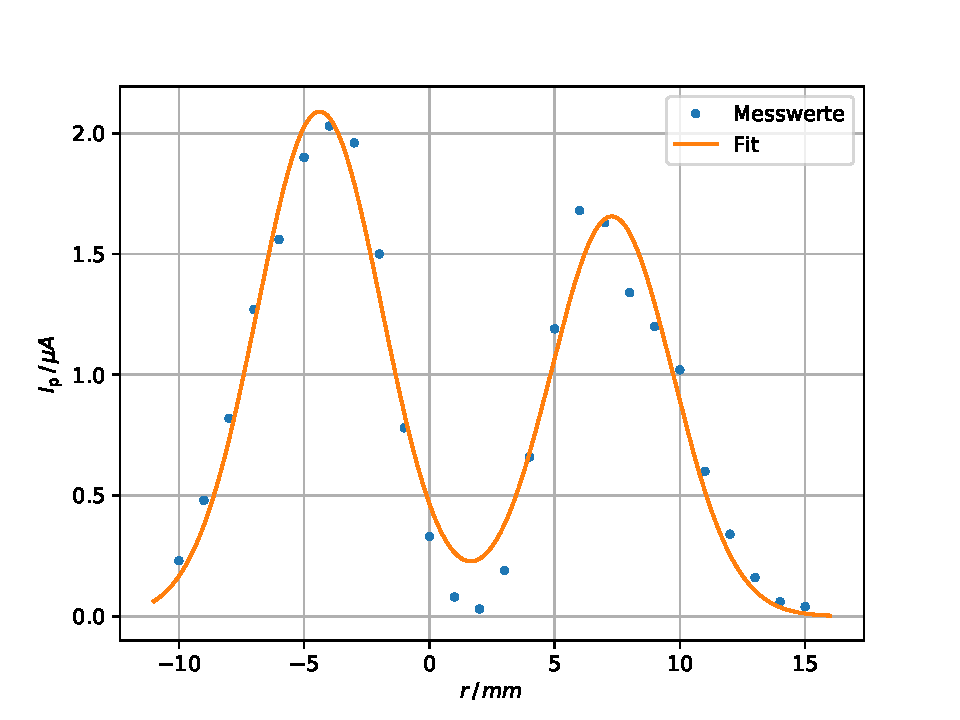
\includegraphics[width=0.8\textwidth]{../Messdaten/plots/T_10.pdf}
  \caption{Plot der in Tabelle \ref{tab: T_10} gelisteten Messwerte. Zusätzlich ist in der Grafik die bestimmte Ausgleichsgeraden zu sehen.}
  \label{fig: T_10}
\end{figure}
\FloatBarrier
\subsection{Auswertung der Polarisation}

In der Tabelle \ref{tab: pola} sind die notierten Werte der Polarisationsmessung
aufgelistet.
\FloatBarrier
\begin{table} 
\centering 
\caption{Aufgenommene Werte bei der Polarisationsmessungs.} 
\label{tab: pola} 
\begin{tabular}{S S S S S S S S S } 
\toprule  
{$\varphi / \si{ \degree }$} & {$\varphi / \si{ \radian }$} & {$I_p / \si{ \milli\ampere}$} & {$\varphi / \si{ \degree }$} & {$\varphi / \si{ \radian }$} & {$I_p / \si{ \milli\ampere}$} & {$\varphi / \si{ \degree }$} & {$\varphi / \si{ \radian }$} & {$I_p / \si{ \milli\ampere}$} \\ 
\midrule  
0 & 0.00 & 0.36 & 130 & 2.27 & 0.75 & 260 & 4.54 & 0.21\\ 
10 & 0.17 & 0.23 & 140 & 2.44 & 0.74 & 270 & 4.71 & 0.34\\ 
20 & 0.35 & 0.12 & 150 & 2.62 & 0.69 & 280 & 4.89 & 0.47\\ 
30 & 0.52 & 0.04 & 160 & 2.79 & 0.61 & 290 & 5.06 & 0.58\\ 
40 & 0.70 & 0.00 & 170 & 2.97 & 0.51 & 300 & 5.24 & 0.67\\ 
50 & 0.87 & 0.01 & 180 & 3.14 & 0.36 & 310 & 5.41 & 0.74\\ 
60 & 1.05 & 0.06 & 190 & 3.32 & 0.24 & 320 & 5.59 & 0.76\\ 
70 & 1.22 & 0.16 & 200 & 3.49 & 0.14 & 330 & 5.76 & 0.73\\ 
80 & 1.40 & 0.28 & 210 & 3.67 & 0.06 & 340 & 5.93 & 0.64\\ 
90 & 1.57 & 0.41 & 220 & 3.84 & 0.01 & 350 & 6.11 & 0.52\\ 
100 & 1.75 & 0.50 & 230 & 4.01 & 0.00 & 360 & 6.28 & 0.39\\ 
110 & 1.92 & 0.62 & 240 & 4.19 & 0.03 &  &  & \\ 
120 & 2.09 & 0.71 & 250 & 4.36 & 0.10 &  & & \\ 
\bottomrule 
\end{tabular} 
\end{table}

An die Messwerte wird die Funktion

\begin{equation}
  \label{eq: func_polarisation}
  I(\phi)=I_0\sin\left(\phi-\phi_0\right)
\end{equation}
mit den folgeden Parametern gefittet:

\begin{align}
  \label{eq: fit_pola}
  \begin{aligned}
  I_0&=\SI{0.748\pm0.005}{\milli\ampere}\\
  \phi_0&=\SI{0.792\pm0.006}{\radian}
\end{aligned}
\end{align}
Die Messwerte und die Ausgleichkurve sind in Abbildung \ref{fig: pola} skizziert.

\begin{figure}[h!]
  \centering
  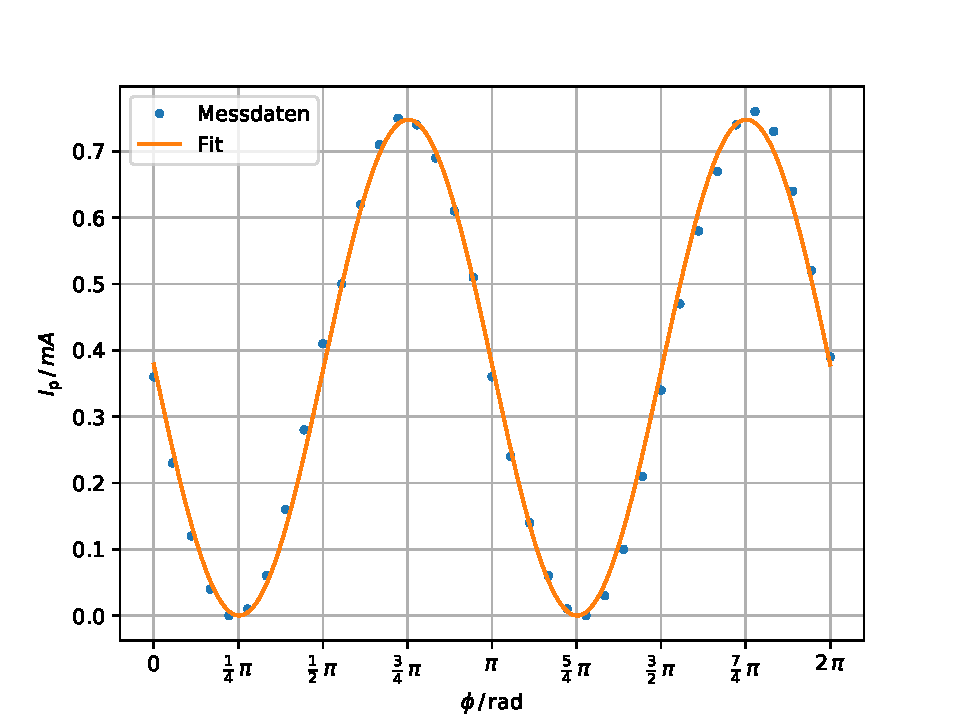
\includegraphics[width=0.8\textwidth]{../Messdaten/plots/pola.pdf}
  \caption{Plot der in Tabelle \ref{tab: pola} gelisteten Messwerte. Zusätzlich ist in der Grafik die bestimmte Ausgleichsgeraden zu sehen.}
  \label{fig: pola}
\end{figure}
\FloatBarrier

\subsection{Wellenlängenbestimmung}
Die für die Bestimmung der Wellenlänge des Lasers aufgenommenen Messwerte sind
in der Tabelle \ref{} notiert.
